% Generated by paper/build_manuscript.py.
\documentclass[10pt]{article}
\usepackage[margin=0.8in]{geometry}
\usepackage[T1]{fontenc}
\usepackage[utf8]{inputenc}
\usepackage{lmodern}
\usepackage{microtype}
\usepackage{graphicx}
\usepackage{booktabs}
\usepackage{array}
\usepackage{amsmath,amssymb}
\usepackage{caption}
\usepackage{enumitem}
\usepackage[numbers,sort&compress]{natbib}
\usepackage[hidelinks]{hyperref}
\usepackage{xcolor}
\definecolor{qnavy}{HTML}{193552}
\definecolor{qblue}{HTML}{2E74B5}
\setlength{\parindent}{0pt}
\setlength{\parskip}{0.55em}
\setlist{nosep,leftmargin=1.4em}
\captionsetup{font=small,labelfont=bf}
\title{\textbf{Exact Real Controls Overturn an Apparent Complex-Valued Robustness Advantage}\\[0.5em]\large A preregistered falsification study across synthetic sequential task families}
\author{Samyar Shafiee\\\small Independent Researcher · Toronto, Canada}
\date{Research manuscript · v1.0.0 · 14 August 2026}
\begin{document}
\maketitle
% Generated from paper/source. Do not edit by hand.
\begin{abstract}
Clinical reasoning is sequential: evidence arrives with sign, absence, timing, and context, while a differential diagnosis should remain revisable until the evidence is sufficient. We investigate whether representing diagnostic hypotheses as an explicitly evolving complex state offers a useful inductive bias for this setting. Q-Neuro maps each observed finding to a low-rank evidence-conditioned operator, composes those operators in observed order, and measures diagnosis probabilities from squared complex amplitudes. The construction is quantum-inspired mathematics implemented on ordinary hardware; it is neither a quantum computer nor a physical model of cognition or disease.

We introduce NeuroWorld, a fully synthetic causal benchmark with chronology twins, factorial disease mechanisms, explicit missingness, unseen generator worlds, irreducible ambiguity, active evidence acquisition, omitted diseases, hidden syndromes, and counterfactual pairs. Across 26 registered studies---25 complete and one preserved failure---we compare Q-Neuro with unordered, recurrent, attention, state-space, associative, graph, real-operator, two-channel real, Hamiltonian-style, dissipative, attractor, tensor, and density-state controls. In a five-world severity sweep at 1,000 training cases, the complex operator exceeds the strongest tested two-channel real control by 0.054--0.063 absolute top-1 accuracy, with world-level 95\% intervals above zero. Critical ablations show that noncommutative order, phase-sensitive readout, and observed-negative evidence each contribute to this result.

The same program identifies decisive boundaries. A tuned GRU is substantially more sample-efficient in the source world; a real operator represents irreducible ambiguity far better; source-fitted temperature scaling worsens shifted calibration; hidden-syndrome and omitted-disease separation are not uniquely complex; phase-coded gradient optimization does not improve the frontier; and a velocity-based hard exit collapses to fixed two-step truncation rather than adaptive reasoning. Frozen-state probes recover simulator factors, but conventional recurrent controls recover them as well or better. The principal contribution is therefore not a claim of clinical or quantum advantage. It is a falsification-led, reproducible framework for testing hypothesis-state computation under causal shift, together with a bounded empirical finding: under the tested synthetic worlds, ordered complex dynamics improve robustness while paying measurable costs in calibration, compute, and ambiguity.

\textbf{Keywords:} complex-valued neural networks; diagnostic reasoning; causal simulation; distribution shift; noncommutative operators; uncertainty; reproducible machine learning

\end{abstract}

\tableofcontents
\clearpage
% Generated from paper/source. Do not edit by hand.
\section{Introduction}
Claims about a new neural representation are only as strong as the control that could have produced the same computation. This is especially important for complex-valued models. Their states can express magnitude and phase compactly, and complex multiplication naturally represents rotations and ordered transformations. Yet a complex linear map also has an exact structured representation over twice as many real coordinates. A comparison against an ordinary real recurrent cell, or against two real channels that are not coupled by the corresponding block matrix, cannot identify whether any observed advantage comes from complex arithmetic, from a structured constraint, from optimization, or simply from an underpowered control.

Q-Neuro began with a positive result. In a family of synthetic sequential reasoning environments called NeuroWorld, an ordered complex operator was more robust under declared causal shifts than several then-tested controls. At moderate shift the mean complex-minus-two-channel-real difference was +0.0602 top-1 accuracy across five worlds. The result replicated within that simulator, and destructive phase interventions showed that the trained model used its phase degrees of freedom. Neither observation established that complex arithmetic was necessary. Both remained compatible with a real structured implementation and with stronger real sequence models.

We therefore reorganized the project around a falsification-first question: \textbf{does the complex operator retain a practically relevant advantage when compared with an exact real implementation and a cellwise best-real envelope on task families not used to formulate the claim?} The answer within the executed scope is no. The exact real block matches the complex computation at numerical precision. Once it is admitted to the comparator set, the sign of the performance gap reverses in a power pilot, in reduced discovery, and in held-out reduced confirmation. A quantitative candidate law that appeared accurate in discovery fails its frozen held-out thresholds. Finally, the preregistered grand benchmark is not opened because the program has not completed the full comparator, search-budget, compute-accounting, shift-grid, and raw-prediction requirements.

This paper makes four bounded contributions. First, it gives an implementation-level exact-real falsifier for the Q-Neuro operator and verifies mapped equivalence across independent task families. Second, it constructs eight nonmedical sequential generator families and a severity-indexed shift surface so that discovery and confirmation can be separated by generator family rather than by random examples alone. Third, it preserves a prospective law failure without refitting and a grand-experiment stop decision without weakening the gates. Fourth, it releases a machine-readable claim ledger that pairs every conclusion with counterevidence, scope, uncertainty, and a prospective falsifier.

The work does not claim clinical validity, universal superiority of real networks, or evidence for a physical quantum process in cognition. The independent studies are deliberately reduced relative to the full preregistration: only five model families were trained, search used one configuration per model, training sizes were restricted, per-trial FLOPs and optimizer steps were not preserved, and raw predictions were not stored. These limitations block the grand experiment and external-validity claims. They do not alter the exact algebraic control or the observed absence of a complex advantage in the executed cells. The resulting paper is a case study in how a project can become scientifically stronger when its favored hypothesis fails.

% Generated from paper/source. Do not edit by hand.
\section{Related work}
\subsection{Complex and structured recurrence}
Trainable complex-valued neural networks, including complex initialization, normalization, convolution, and recurrent components, are established methods rather than a Q-Neuro invention \citep{trabelsi2018}. Complex and unitary recurrent networks were developed to stabilize long-range dynamics and represent rotations efficiently \citep{arjovsky2016,jing2017}. Real orthogonal recurrence offers a closely related norm-preserving alternative and has shown that carefully structured real models can outperform some unitary controls with fewer parameters \citep{helfrich2018}. These precedents make a broad complex-versus-real comparison scientifically insufficient.

Arjovsky and colleagues explicitly describe the real two-channel representation of a complex unitary matrix \citep{arjovsky2016}. For the present study, that known identity is not a novelty claim; it is an adversarial control. More recent theory reinforces why arithmetic, parameterization, and optimization should be separated. Infinite-width analyses show that common real-valued backpropagation can collapse many complex-network training dynamics toward ordinary real dynamics \citep{tan2022}. Conversely, theoretical settings exist in which a complex neuron represents functions unavailable to a finite-width two-layer real network while learning some real targets more slowly \citep{wu2023}. Capacity bounds for modReLU networks also begin from the standard identification of complex coordinates with paired real coordinates \citep{altunoren2026}. Our negative result is therefore architecture-specific, not a theorem that complex models can never help.

\subsection{Quantum-inspired state and order effects}
Quantum probability has been used to model human question-order and causal-reasoning effects through noncommuting projections and contextual state updates \citep{wang2014,trueblood2012}. Hidden quantum Markov models and density-matrix-inspired language models further demonstrate that quantum-mathematical state representations can be useful without implementing physical quantum hardware \citep{srinivasan2018,yan2024}. Q-Neuro uses related mathematical motifs - ordered updates, phase-sensitive state, and magnitude-squared readout - but makes no inference about physical quantum cognition. Noncommutativity is a property of the computation, not evidence about its substrate.

\subsection{Modern sequence controls and uncertainty}
Structured state-space models provide efficient long-sequence dynamics and form an important real-valued comparator family \citep{gu2022}. Gated recurrent units, orthogonal recurrence, and unrestricted real operators address different inductive biases and optimization surfaces. Calibration and out-of-distribution detection require separate evaluation because high top-1 accuracy does not imply reliable confidence \citep{guo2017,hendrycks2017}. Q-Neuro consequently records negative log-likelihood, expected calibration error, and Brier score alongside top-1 accuracy, although the present primary falsifier is top-1 performance against the cellwise best-real envelope.

\subsection{Position of the present work}
The publishable object is not a new complex algebra. It is a fully traceable reversal of an architectural interpretation. A positive within-simulator result is retained, its insufficient comparator is named, an exact control is implemented, new task families are generated before confirmation, a candidate relationship is frozen, and failed readiness gates stop a sealed test. This sequence differs from an ordinary ablation study because the unfavorable result controls which claims are permitted and which experiment may legally execute. Whether that workflow is novel in the literature requires peer review; no priority claim is made here.

% Generated from paper/source. Do not edit by hand.
\section{Mathematical framework}
\subsection{Complex hypothesis-state update}
Let a tokenized observation at step t be embedded as a real vector x\_t. The implemented complex operator maintains h\_t in C\textasciicircum{}d and applies a token-conditioned update followed by a phase-compatible nonlinearity and a magnitude-sensitive readout. Suppressing low-rank factorization and bias terms, the linear part is

\begin{equation}
h_t = W_t h_{t-1} + U x_t
\end{equation}

Write h = a + ib and W = A + iB, with a, b real vectors and A, B real matrices. Then the same multiplication is

\begin{equation}
\begin{bmatrix}\Re(Wh)\\\Im(Wh)\end{bmatrix}=\begin{bmatrix}A&-B\\B&A\end{bmatrix}\begin{bmatrix}a\\b\end{bmatrix}
\end{equation}

This is an identity, not an approximation. The exact real block has the same real degrees of freedom as W because the four blocks are tied by A and B. When initialization, token order, loss, and optimizer policy are mapped consistently, any prediction difference beyond numerical tolerance is an implementation failure or a consequence of a non-mapped operation, not evidence for uniquely complex capacity.

\subsection{Three distinct hypotheses}
The comparator audit separates three hypotheses that are often conflated.

\begin{itemize}
\item \textbf{Representational uniqueness:} the complex model computes a function unavailable to the exact structured real block.
\item \textbf{Parameterization advantage:} the complex coordinates create a more useful inductive bias or optimization trajectory even though the represented mapped function class overlaps.
\item \textbf{Architecture advantage:} the complete complex operator outperforms all parameter- and compute-matched real sequence architectures on the prespecified outcome.
\end{itemize}

The algebra directly falsifies representational uniqueness for the mapped linear complex operations. Empirical mapped runs test whether the implementation preserves that identity through the complete network. The best-real envelope tests architecture advantage over the real models actually evaluated. Parameterization advantage remains a legitimate possibility in other objectives, initializations, nonlinearities, or training regimes; it is not supported by the present top-1 results.

\subsection{Primary estimand}
For family f, training size n, training seed s, world w, and severity q, let A\_C(f,n,s,w,q) be complex top-1 accuracy. Let R be the prespecified set of evaluated real controls. The nested effect is

\begin{equation}
\Delta_{fnswq}=A_C(f,n,s,w,q)-\max_{r\in\mathcal{R}}A_r(f,n,s,w,q)
\end{equation}

This cellwise envelope is intentionally adversarial. It asks whether the candidate beats the strongest real alternative in each matched condition, not whether it beats a conveniently chosen average control. It also creates selection optimism for the real side, which is acceptable for a falsifier but must be acknowledged when interpreting magnitude.

\subsection{Structural predictors and candidate law}
Each generator world exposes two preregistered structural descriptors: empirical mutual information between observed order and the target, and shift severity q. Six candidate families were compared on discovery aggregates. The selected quadratic candidate was

\begin{equation}
\widehat{\Delta}=\beta_0+\beta_1 I+\beta_2 q+\beta_3 I^2+\beta_4 Iq+\beta_5 q^2
\end{equation}

The coefficients were frozen before held-out family evaluation. Passing required R2 at least 0.50, sign accuracy at least 0.80, and mean absolute error at most 0.015. A fit to discovery data was not itself treated as a law.

\subsection{Claim rule}
The preregistered practical threshold for a favorable complex effect was +0.02 top-1. Because the executed independent profiles deviate from the full protocol, they are outcome-ineligible for the strongest confirmatory category even if a threshold were crossed. Exact equivalence, empirical effect direction, and law failure are reported separately rather than collapsed into one verdict.

% Generated from paper/source. Do not edit by hand.
\section{Architecture}
\subsection{Evidence representation}
NeuroWorld emits 40 binary findings, demographic context, explicit observation masks, and an observed sequence. A positive observation and a negative observation use distinct token identities; a missing finding supplies no token. Each token carries normalized time and may be accompanied by a context-conditioned injection. This representation prevents the common leakage-prone shortcut of coding “not observed” as “observed absent.” Unordered baselines receive the same information content through separate positive, negative, and missing channels, but not the chronology needed to solve order twins.

The complex operator state uses a learned initial vector, evidence embeddings, evidence-specific diagonal actions, and factorized low-rank transformations. Low-rank factors keep the parameter count near 20,000 real scalars, comparable to the small baselines. The real operator uses the same sequence interface. The two-channel real model receives paired state channels and a quadratic readout so that extra width and squared measurement are not mistaken for a uniquely complex effect.

\subsection{Conventional controls}
The comparison suite includes logistic regression, an unordered MLP, a tiny Transformer, a validation-tuned GRU, and a diagonal state-space model. Logistic regression and the MLP establish performance available from aggregated evidence. The Transformer tests attention over observed order at a similar scale. The GRU supplies a strong recurrent inductive bias and is tuned only on source validation NLL. The diagonal state-space model tests compact linear recurrence with learned input and nonlinear readout.

The full-data chronology task saturates for all ordered controls, so it is treated as a correctness check. The low-data and shifted worlds carry the architectural comparison. This distinction was introduced after the original baseline set proved too weak: the tuned GRU reverses the apparent source-world sample-efficiency advantage of the operator models, while becoming fragile under generator shift. Preserving that reversal is central to the architecture story.

\subsection{Mechanism families}
Eighteen laws are evaluated in the broad mechanism suite. In addition to the conventional and operator models, these include a complex MLP, modern-Hopfield-style retrieval, a declared factor-graph network, a multiplicative coupled-tensor model, energy and adaptive attractors, Hamiltonian-style evolution, elementwise dissipation, their hybrid, and low-rank density dynamics. The graph control uses the simulator’s coarse factor grouping but not label-specific causal probabilities; its poor result warns that broad causal alignment is not equivalent to learning the generator.

Associative and attractor models intentionally sum or pool evidence before iterative inference, so failure on chronology pairs is expected. That failure is useful: it verifies that the counterfactual task reacts to an architectural invariance rather than merely rewarding model size. Hamiltonian and complex operator laws retain order. Density dynamics also retain a sequential state, but its diagnosis-space factorization and diagonal measurement create a different ambiguity--robustness compromise.

\begin{figure}[t]
\centering
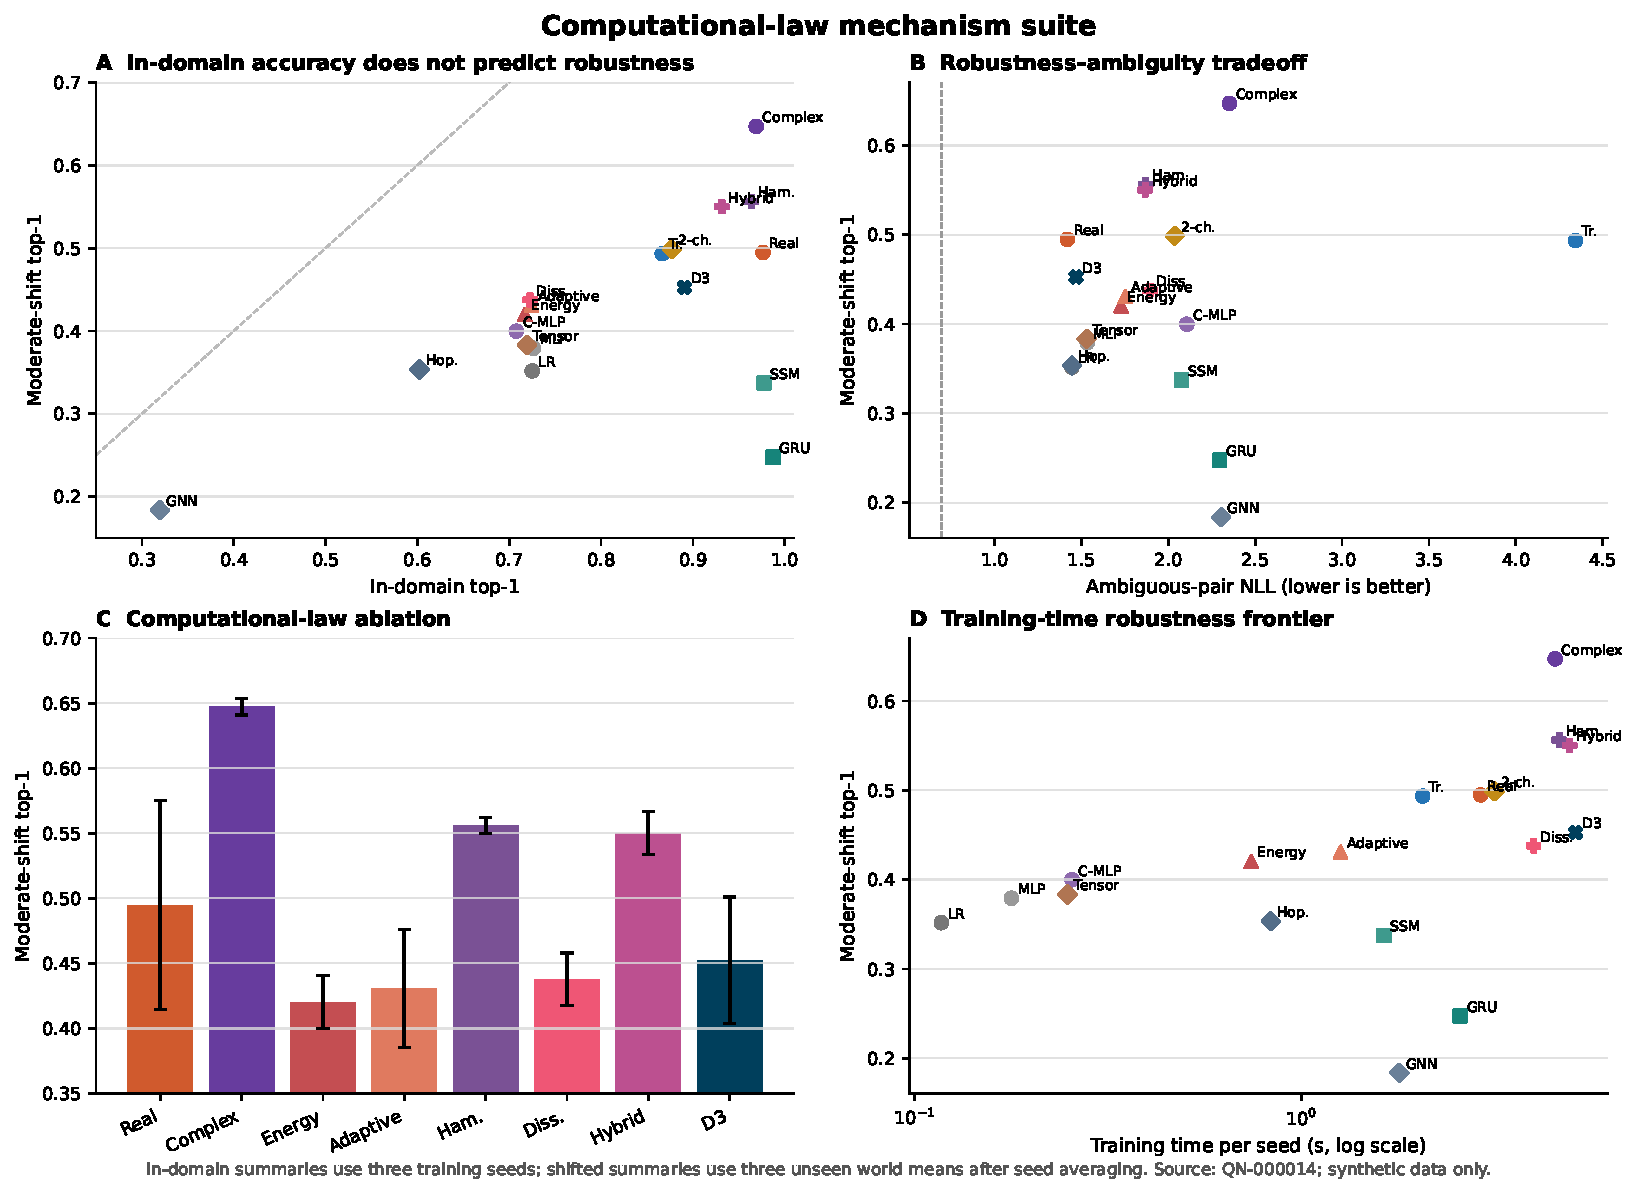
\includegraphics[width=0.98\linewidth]{figures/dynamics_suite.pdf}
\caption{Eighteen computational laws occupy different positions in source accuracy, unseen-world robustness, ambiguity, and chronology-pair performance. No single family dominates every objective.}
\label{fig:dynamics_suite}
\end{figure}

\subsection{Parameter and compute matching}
Most neural architectures are configured near 20,000 trainable real scalars. Complex parameters count as two real scalars. Some controls are smaller by design: logistic regression has 1,660 parameters, while the density model is approximately 16,240. Parameter matching does not imply compute matching. Complex multiplication and evidence-specific operators are slower than the MLP and often slower than the real control on CPU. Training time, process memory, and inference latency are therefore measured separately.

Peak RSS values are interpreted cautiously because sequential in-process runs can reuse allocator caches. Wall-clock times are machine-specific and only compare runs on the same hardware and code path. The public artifacts include environment and configuration records so that external replication can distinguish algorithmic trends from one-machine timing.

\subsection{Architectural invariants}
Unit tests and experiment-time checks enforce that padding does not evolve a state, complex probabilities are finite and normalized, state norms remain bounded, counterfactual pairs differ only in the declared causal factor, and density matrices are Hermitian, positive semidefinite, and unit trace within tolerance. A synthetic nonzero-commutator test confirms that swapping two learned operators can change state. These checks validate implementation properties; they do not show that the learned noncommutativity is causally responsible for every performance difference.

\subsection{Architecture selection after falsification}
The most defensible architectural object at the end of the study is the simple complex operator, not the most elaborate dynamical proposal. Pure Hamiltonian evolution is competitive under shift, but remains below the complex operator. Adding generic dissipation does not help. Increasing density rank does not help. The adaptive attractor does not produce meaningful case-dependent depth. The coupled tensor and graph controls do not approach the robustness frontier. This result argues for retaining the smallest law that survives the declared ablations while treating more ornate mechanisms as negative evidence.

The selected architecture should still not be called “the best model.” The GRU is better at extreme source-world sample efficiency, the real operator is much better on irreducible ambiguity, and several conventional states support stronger linear factor probes. Q-Neuro’s value is conditional: within the tested synthetic family, it combines high chronology accuracy with the strongest moderate-shift top-1 result. Its costs remain visible in every summary.

% Generated from paper/source. Do not edit by hand.
\section{Training and model selection}
\subsection{Shared optimization protocol}
Independent-task models were trained on CPU with AdamW, batch size 128, learning rate 0.001, weight decay 0.0001, at most six epochs, and patience three. Five fixed training seeds were used in discovery and five new seeds in held-out evaluation. Model selection used source-world validation data only. Each trained checkpoint was evaluated without adaptation across the registered shifted worlds and severities.

Discovery used training sizes 250 and 1,000. Held-out evaluation used size 1,000. The original full protocol additionally required 5,000 and 25,000 examples, a primary grand-test size of 5,000, and a substantially larger hyperparameter search. Because those conditions were deferred, the independent studies are labeled reduced and outcome-ineligible throughout this paper.

\subsection{Comparator selection within evaluation cells}
For each family, training size, training seed, world seed, and severity, the best-real model was selected by top-1 accuracy within that same cell. Ties were resolved deterministically by model name. This procedure is transparent and reproducible, but it is more stringent than selecting a single real model globally. Its role is to challenge the complex-advantage claim, not to estimate the expected performance of a deployed model-selection procedure.

\subsection{Calibration and auxiliary metrics}
Each evaluation records top-1 accuracy, NLL, expected calibration error, Brier score, and separate accuracy for order-dependent and non-order-dependent examples where defined. Counterfactual order pairs were also generated for structural checks. The primary effect in the current falsification analysis is top-1 accuracy; calibration metrics are descriptive because no favorable complex primary effect survived to support a secondary claim.

\subsection{Reproducibility controls}
Every run reserved an immutable result directory, stored its configuration and environment record, and registered its hypothesis and preregistration identifiers in SQLite. The pipeline rejected dirty worktrees for evidence-generating runs unless an explicitly ineligible smoke mode was used. Discovery and confirmation used disjoint family names, world seeds, training seeds, and configuration files. The frozen law artifact stores code and configuration hashes as well as the commit preceding held-out execution.

\subsection{Deferred compute accounting}
The repository preserves CPU device selection and runtime environment, but the reduced studies do not contain per-trial FLOPs or optimizer-step records. Search budgets also favor neither side because each executed model received one configuration, yet this is not the prospectively required equal-or-real-favoring search. These missing records are reported as blockers rather than estimated after the fact.

% Generated from paper/source. Do not edit by hand.
\section{NeuroWorld}
\subsection{Causal simulator}
NeuroWorld is a synthetic environment for testing diagnostic reasoning mechanisms without patient data. It defines 20 diagnosis archetypes and 40 findings organized around mechanism, localization, temporality, and context. Each diagnosis specifies factor-dependent finding probabilities, demographic tendencies, and an observation process. Cases are sampled from the causal template, then findings are observed, signed, timestamped, and possibly omitted. The generator emits latent factors so that representation probes and exact interventions are possible.

The simulator is not intended to mimic epidemiology, coding practice, or the full complexity of neurology. Disease names are abstract labels and findings are synthetic variables. “Neurological” describes the structure of the reasoning problem---mechanism, localization, time course, context, and differential competition---not clinical fidelity. The benefit is control: chronology, missingness, nuisance evidence, ambiguity, and new syndromes can be manipulated without harming people or leaking protected data.

\subsection{Chronology twins}
Four labels form two chronology-twin pairs. Members of a pair share aggregate evidence and demographics; two marker events occur in opposite order. Standard random cases may hide one or both markers under the observation process. A separate counterfactual set exposes both markers and varies only order. An unordered model should average the twins and obtain zero pair accuracy in expectation, whereas a valid ordered model can solve both.

Unit tests verify that paired records have equal signed evidence multisets, identical non-temporal covariates, and only the declared ordering difference. Complete-order accuracy is reported separately from all-case top-1. This prevents an architecture from receiving credit for predicting easier factorial cases while ignoring chronology.

\subsection{Factorial diagnoses and held-out composition}
The remaining diagnoses combine mechanism, localization, temporality, and context factors. A held-out composition split removes selected positive-finding conjunctions from training and requires one at test time. The task checks whether a model can recombine familiar individual factors. At 3,000 cases it saturates for several architectures and therefore fails as a discriminator. A stronger future version should reduce data and introduce inseparable tensor or XOR-like interactions with parameter-matched multiplicative controls.

\subsection{Missingness and signed evidence}
Observation is generated explicitly rather than imputing every unobserved finding as negative. Positive findings and observed absences are separate tokens; unobserved findings are omitted. Shift worlds can reduce observation rate, add timestamp jitter, mix probabilities toward 0.5, change nuisance findings, and lower the chance that chronology markers appear. The model is therefore tested both when the causal relation is visible and when the observation process obscures it.

\subsection{Unseen worlds}
The initial shift replication uses a nuisance-seed world and a noisy/sparse world. The confirmation suite declares five unseen world seeds at four severities: nuisance, mild, moderate, and severe. The disease-factor scaffolding remains related, but secondary findings, nuisance evidence, probability noise, sparsity, and temporal jitter vary. These are genuine held-out generator instantiations, though not independently designed simulators.

\begin{figure}[t]
\centering
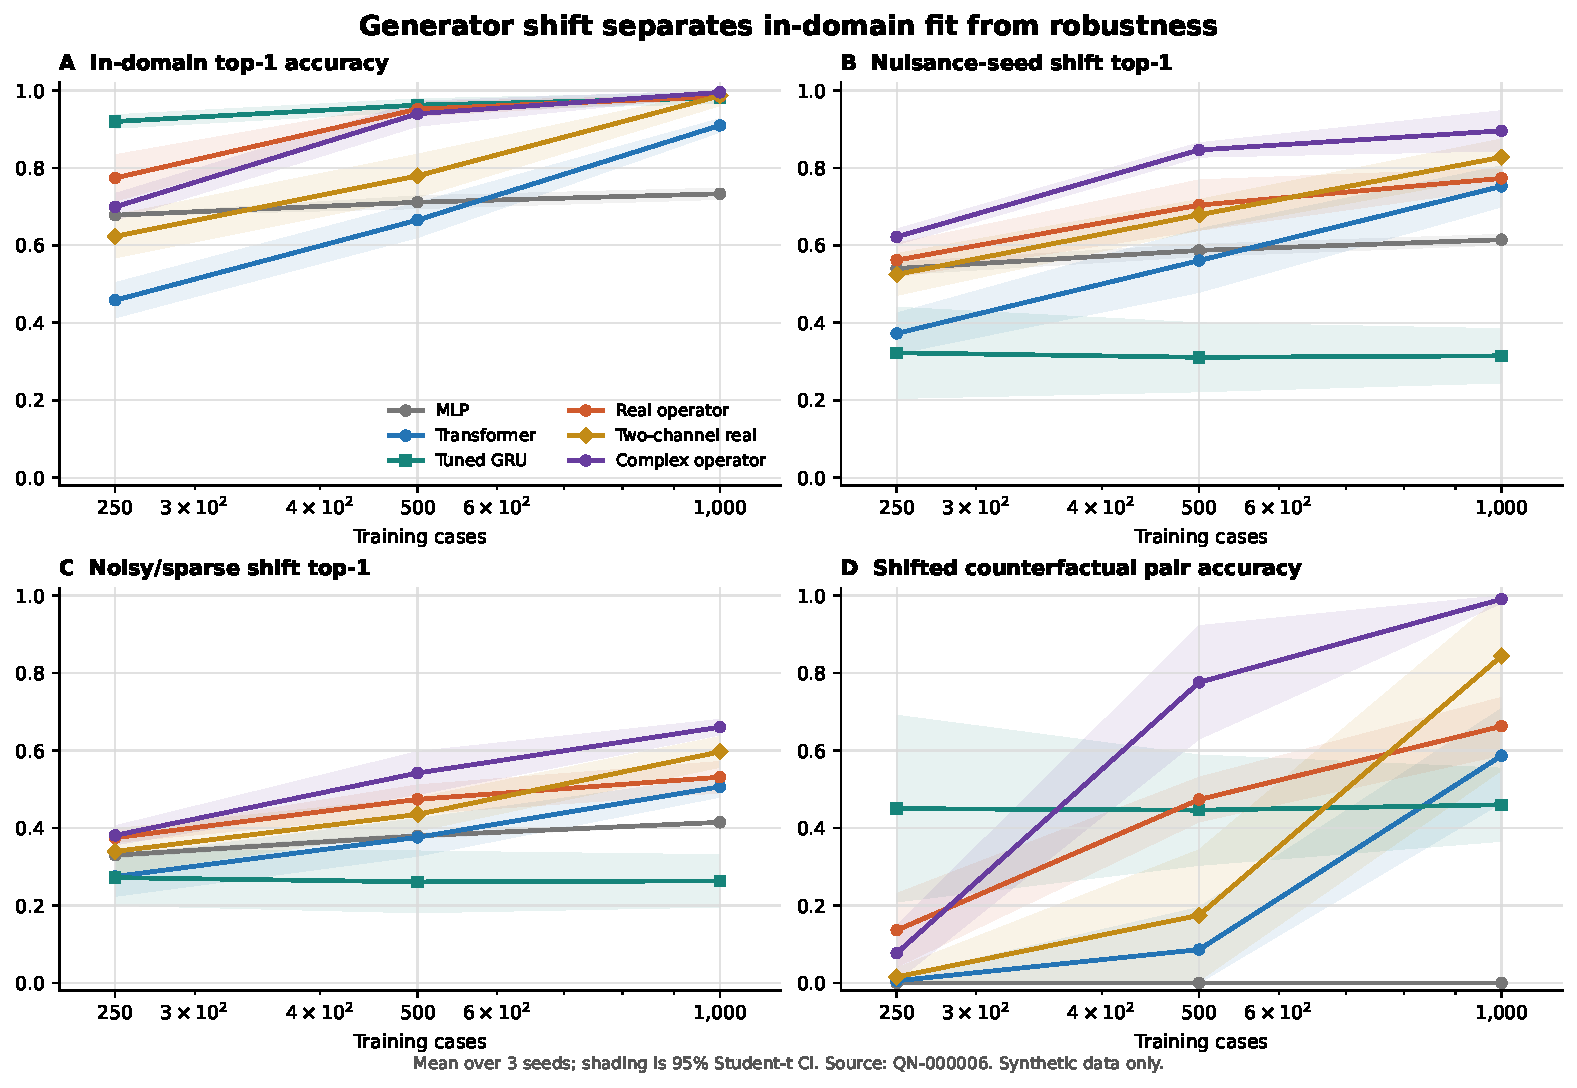
\includegraphics[width=0.98\linewidth]{figures/generator_shift_replication.pdf}
\caption{The stronger-control replication separates source-world fit from robustness. A tuned GRU is strongest at very low source data but collapses under the declared generator shifts; the complex operator becomes strongest under nuisance and noisy/sparse shift at 1,000 cases.}
\label{fig:generator_shift_replication}
\end{figure}

\subsection{Ambiguity, omitted labels, and hidden syndromes}
Irreducible ambiguity pairs present identical observations with two valid chronology labels. The ideal prediction assigns all mass equally to the twins, giving pair NLL log(2). This benchmark tests whether a differential remains calibrated when the label is unidentifiable. It is distinct from standard uncertainty on difficult but identifiable cases.

The omitted-disease task removes one label entirely during training and evaluates whether confidence or representation distance separates it from known cases. The hidden-syndrome task creates an unlabeled cross-factor signature and measures representation separation. Neither task claims disease discovery. High AUROC only shows that a synthetic construct lies away from known examples under a declared score.

\begin{figure}[t]
\centering
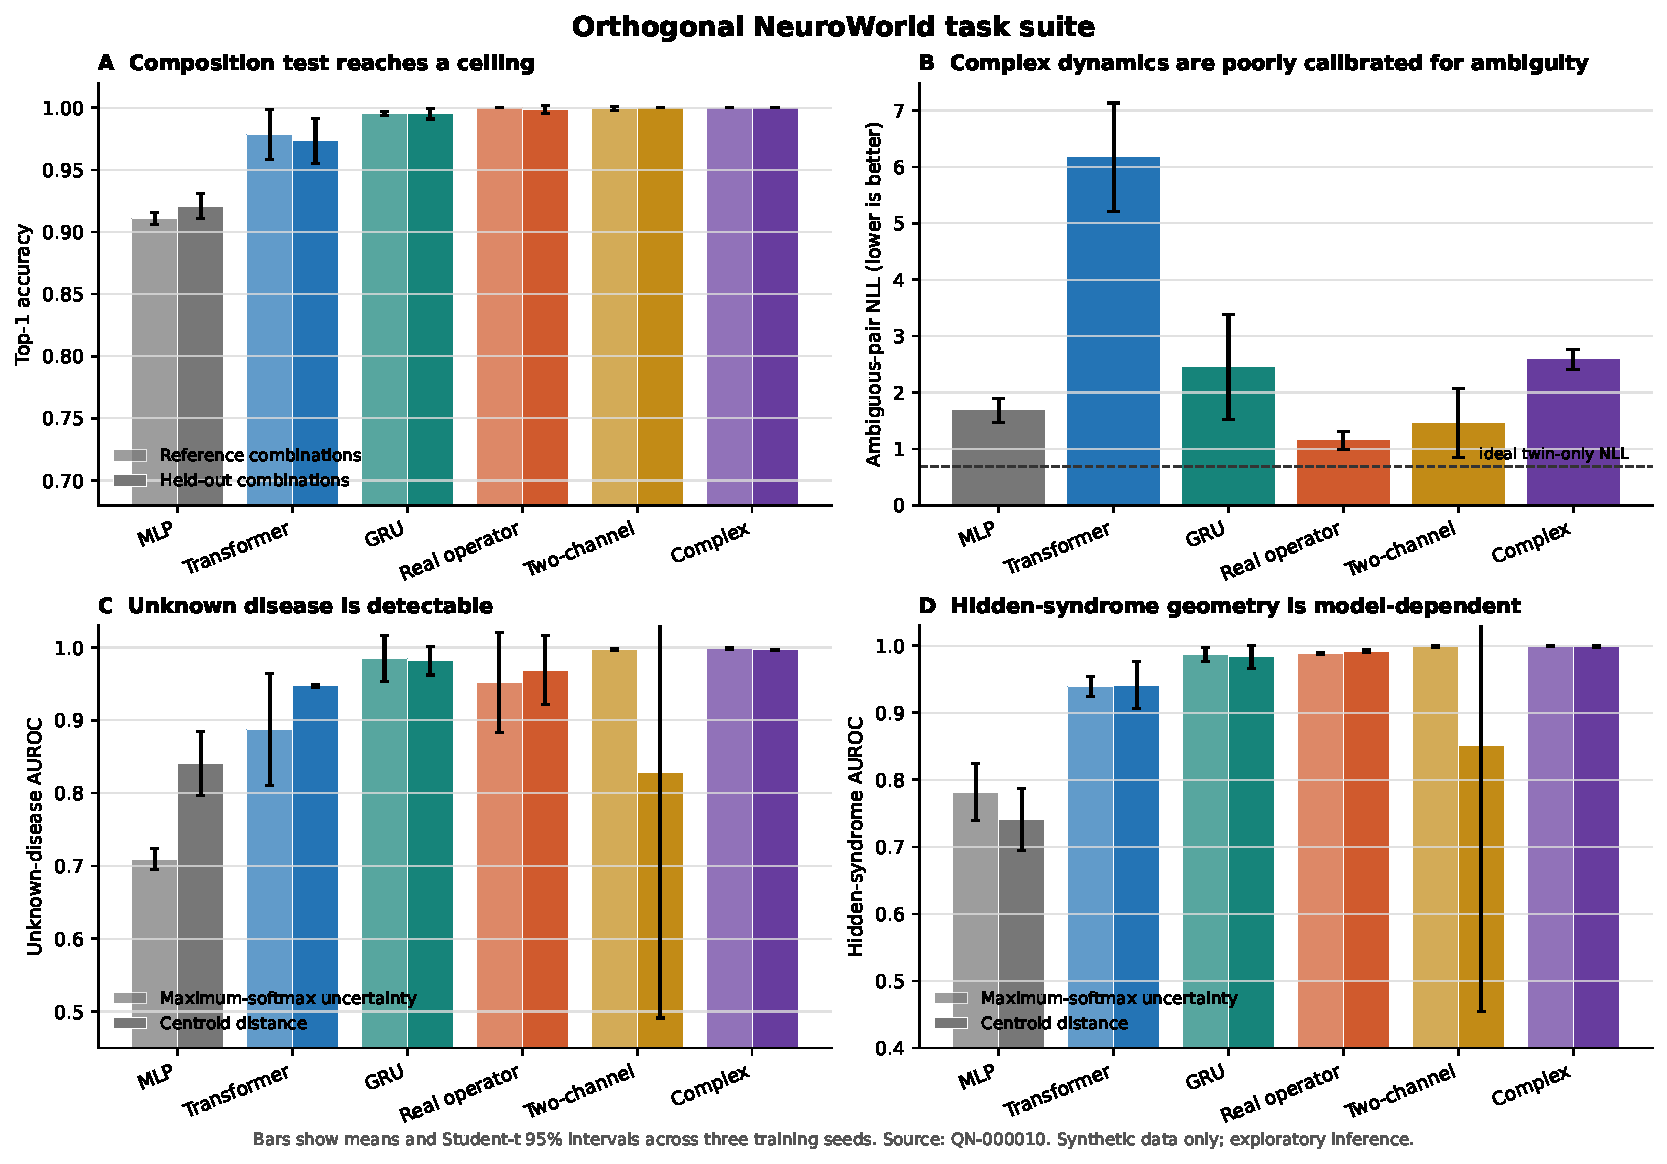
\includegraphics[width=0.98\linewidth]{figures/neuro_task_suite.pdf}
\caption{The orthogonal task suite separates composition, ambiguity, omitted-disease rejection, and hidden-syndrome representation tests. Success on one axis does not imply success on the others.}
\label{fig:neuro_task_suite}
\end{figure}

\subsection{Active evidence acquisition}
For active acquisition, the complete set of 40 binary outcomes exists but a policy reveals one at a time. Query costs are equal. Random order, fixed mutual-information order, and model-conditioned expected entropy reduction are evaluated from one to twelve queries. Accuracy AUC is the average top-1 across those budgets, not receiver-operating-characteristic area. This task excludes chronology twins so that a set-based query policy is not asked to infer event order from unordered acquisition.

The simulator does not model the causal dependence among requested tests, the semantics of asking a patient a question, or unequal cost and risk. It is a controlled partial-information benchmark. A clinically meaningful extension would need conditional outcome models, governed cost definitions, and prospective policy evaluation.

\subsection{Leakage and scope controls}
Train, validation, and test cases use disjoint random streams. Model selection never reads shifted test metrics. World seeds are held out before training. Counterfactual pairs are generated separately. The registry stores dataset fingerprints, configuration hashes, seeds, hardware/software environment, and result paths. One early asymmetric-input study is retained but superseded because only the MLP received demographic context; the corrected study equalizes inputs.

NeuroWorld remains a single simulator family built by the same project that proposes Q-Neuro. That is the largest external-validity limitation. Multiple seeds reduce sensitivity to one random template but do not create an independent scientific replication. The benchmark is best viewed as a causal wind tunnel: valuable for mechanism stress tests, insufficient for claims about real patients.

% Generated from paper/source. Do not edit by hand.
\section{Experimental design}
\subsection{Evidence stages}
The next-phase program was organized so that later stages could not rescue earlier failures by changing the estimand.

\begin{enumerate}
\item \textbf{Comparator audit:} reconstruct the historical result and determine whether the two-channel control is algebraically equivalent.
\item \textbf{Exact-equivalence and mechanism tests:} map the complex operator into a tied real block and test forward and outcome agreement; apply destructive phase interventions only as mechanism probes.
\item \textbf{Power pilot:} estimate the number of worlds required for a minimum practical effect of 0.02 without making an outcome claim.
\item \textbf{Reduced discovery:} train five models on four independent generator families; compute cellwise best-real effects; select one law from six prespecified families.
\item \textbf{Freeze:} store coefficients, thresholds, hashes, family split, and a prohibition on using the candidate for the grand outcome.
\item \textbf{Held-out reduced confirmation:} evaluate the frozen law and architecture effect on four untouched families with new seeds.
\item \textbf{Grand preflight:} open no sealed outcome unless every readiness gate passes.
\end{enumerate}

\subsection{Sample structure}
Discovery trained 200 model instances: four families x two training sizes x five training seeds x five models. Their evaluation generated 14,400 metric records and 2,880 complex-minus-best-real nested effects across 24 worlds and three severities. Held-out evaluation trained 100 instances: four families x one training size x five seeds x five models. It generated 9,600 records and 1,920 nested effects across 32 worlds and three severities.

The hierarchical summary gives equal weight to generator family and treats world as the top-level resampling unit, with training-seed observations nested within world. The held-out analysis uses 20,000 bootstrap resamples over four families, 128 worlds, and 640 family-world-seed observations. A two-sided world-level sign-flip test is reported as exploratory because the reduced profile is outcome-ineligible.

\subsection{Frozen decision thresholds}
A favorable architecture result required a positive aggregate effect whose multiplicity-adjusted interval exceeded +0.02. Law confirmation required all three of R2 at least 0.50, effect-sign accuracy at least 0.80, and MAE at most 0.015. The grand experiment required all readiness gates, not a majority vote. The benchmark-access code therefore returned before execution when any mandatory gate failed.

\subsection{Outcome eligibility}
The discovery and held-out studies were intentionally useful but insufficient substitutes for the full program. Their protocol deviations were written into each result artifact: omitted training sizes, incomplete real envelope, one-trial search, incomplete ShiftGauntlet, and no authority to support the strongest outcome category or QN-GRAND-001. We report their numerical results because they are direct evidence about the candidate claim; we do not relabel them as the preregistered grand confirmation.

\subsection{Statistical estimands}
The principal descriptive estimand is mean complex top-1 minus cellwise best-real top-1. We also report the median, trimmed mean, worst decile, and probability of superiority. Exact-real checks use maximum absolute metric differences. The law uses 12 family-by-severity aggregate cells in discovery and 12 in held-out evaluation. All result directories, analysis code, claim text, and figure inputs are distributed with the repository.

% Generated from paper/source. Do not edit by hand.
\section{Results}
\subsection{Comparator identity changes the conclusion}
The historical within-NeuroWorld comparison is positive: complex minus two-channel real at moderate shift is +0.0602 top-1. The stronger comparisons are all non-positive. The QN-000031 power pilot estimates -0.0552 at size 1,000. Reduced discovery estimates -0.0370 against the cellwise best-real envelope. Held-out reduced confirmation estimates -0.00916. These values arise from different task surfaces and are not combined as a meta-analysis. Their joint role is diagnostic: the sign of the conclusion depends on which real comparator and task family are named.

\subsection{Exact real computation reproduces the candidate}
In the held-out study, complex and exact-real top-1 accuracies match in every one of 1,920 nested cells. Maximum absolute differences are 0 for top-1, 3.58 x 10\textasciicircum{}-7 for NLL, and 1.19 x 10\textasciicircum{}-7 for ECE. The earlier mapped mechanism experiment found maximum metric disagreement of approximately 4.8 x 10\textasciicircum{}-7. This replication across four new generator families supports implementation-level equivalence at numerical precision.

The exact-real control wins the best-real selection in 1,478 held-out cells, while the real polar operator wins 442. The complex operator wins none. Because the exact block is constrained to the same mapped structure, these results do not show that an unrestricted real model is inherently better. They show that explicitly complex arithmetic is not required to obtain the candidate's computation and does not create a favorable top-1 effect in the tested training pipeline.

\subsection{Reduced discovery yields no positive effects}
Across 2,880 nested discovery effects, zero are positive and the mean is -0.03695. The result spans four generator families, two training sizes, five training seeds, 24 worlds, and three severities. It is outcome-ineligible because only five models and one search configuration per model were executed. Nevertheless, it provides no empirical basis for advancing an intrinsic complex-advantage claim.

Six structural relationship families were fit to 12 family-by-severity aggregates. The quadratic candidate minimized the prespecified selection proxy, with discovery R2 0.9487 and MAE 0.002604. Its predictors were empirical order-target mutual information and shift severity. The frozen artifact explicitly prohibited a general-law claim and use for the grand outcome.

\subsection{The frozen relationship fails untouched families}
Held-out evaluation contains 1,920 nested effects. Zero are positive, 1,538 are exactly zero at the recorded precision, and the remaining 382 are negative. The mean is -0.009158, median 0, standard deviation 0.02355, 10\% trimmed mean -0.002485, and worst-decile mean -0.04167. Across 128 world summaries, the mean is again -0.009158 and the median is -0.008056.

The hierarchical bootstrap interval is -0.01325 to -0.00457. The exploratory two-sided world sign-flip p value is approximately 5.0 x 10\textasciicircum{}-6. Because the profile is outcome-ineligible, this p value cannot promote the study into the preregistered grand category. It instead quantifies the consistency of a non-positive effect within the executed scope.

The frozen quadratic relationship transfers only the sign. Held-out sign accuracy is 1.0 because both predicted and observed aggregates are non-positive. Magnitude prediction fails: R2 is -30.94 and MAE is 0.03126, violating the frozen R2 and MAE thresholds. No coefficients were changed after this result. QN-LAW-001 is therefore a failed candidate, not a general computational law.

\begin{figure}[t]
\centering
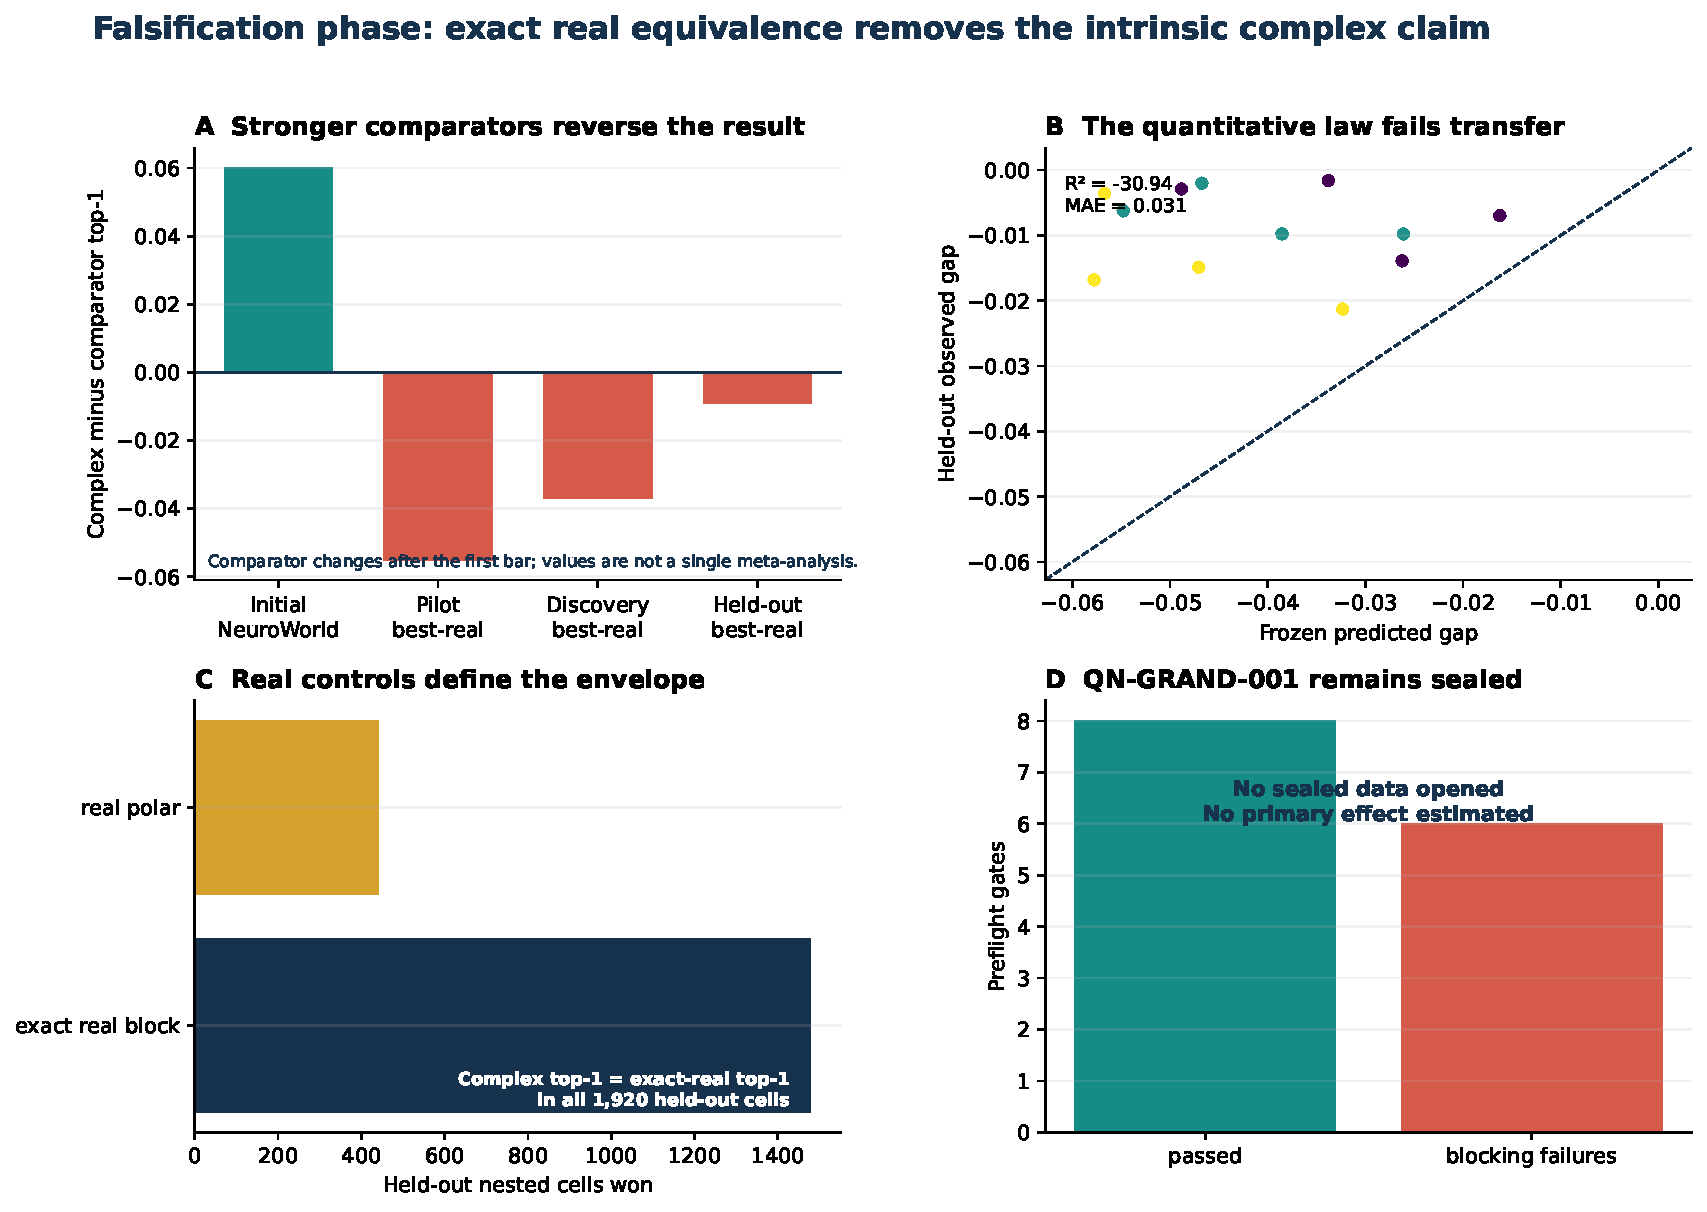
\includegraphics[width=0.98\linewidth]{figures/falsification_phase.pdf}
\caption{Comparator-sensitive effects and prospective stop decisions. The historical positive estimate compares the complex operator with a non-equivalent two-channel real model. Pilot, discovery, and held-out estimates use a best-real envelope that includes the exact block. The held-out interval is a family/world/seed hierarchical bootstrap. The final panel records the failed frozen law and the blocked sealed experiment.}
\label{fig:falsification_phase}
\end{figure}

\subsection{The grand benchmark remains sealed}
QN-GRAND-001 passed eight readiness checks, including the repaired shortcut audit, exact-real equivalence, power planning, frozen-law presence, held-out family separation, and nonmedical scope. It failed six mandatory gates: only 4 of 14 required real controls were present; each evaluated model had one search trial instead of the required 8 or 10; FLOPs and optimizer-step records were missing; the full ShiftGauntlet outcome grid was absent; discovery was reduced rather than full; and raw predictions were not preserved.

The preflight returned \texttt{blocked\_before\_execution}. It records \texttt{executed=false} and \texttt{sealed\_benchmark\_opened=false}, with no primary effect estimate. The stop is a result of the protocol, not an operational accident. Opening the benchmark after a failed gate would convert a prospective test into an exploratory analysis and is deliberately unsupported by the release code.

% Generated from paper/source. Do not edit by hand.
\section{Ablations}
\subsection{Noncommutative order}
The commutative complex accumulator retains a complex state and magnitude-squared readout but sums evidence injections. Its in-domain top-1 is 0.704, moderate-shift top-1 is 0.415, and chronology-pair accuracy is zero. The full complex operator reaches 0.969, 0.647, and 1.000. The paired shift effect is +0.232 with its three-world interval above zero. This is the largest critical ablation and confirms that ordered operator composition, not complex storage alone, is necessary for the leading result.

The control is intentionally algebraic. Because addition commutes, it cannot encode the marker order. A performance collapse on pairs is therefore expected, while the moderate-shift loss shows that chronology-related sequential structure also contributes to the broader shifted set. It remains possible that a different ordered real architecture could reproduce the result; the ablation establishes necessity within Q-Neuro, not exclusivity across all computation.

\subsection{Phase-sensitive measurement}
The two-channel real control reaches 0.499 moderate-shift top-1 and 0.663 pair accuracy. The complex operator adds +0.148 shift accuracy. The phase-insensitive magnitude readout retains the full complex recurrence but forbids destructive readout interference; it reaches 0.543 shift top-1 and 0.825 pairs, leaving a +0.104 gap to the full model. Phase-sensitive measurement is therefore functionally important under the trained law.

This result is stronger than post hoc phase scrambling because the ablated model is retrained. It is still not a theorem about complex arithmetic. A sufficiently general real network can represent complex multiplication using paired channels. The finding is that the tested complex parameterization provides a useful bias relative to the declared controls at this scale.

\subsection{Observed-negative evidence}
Removing the negative-evidence channel reduces shift top-1 from 0.647 to 0.575 and chronology-pair accuracy from 1.000 to 0.972. The +0.072 shift effect has an interval above zero. The ablation also worsens ambiguity NLL to 3.274. Negative findings therefore provide more than missingness; they shape both elimination and uncertainty.

Observed-negative tokens are not yet diagnosis-conditional contradiction operators. They are learned tokens whose effects emerge through supervised training. A stronger causal study would intervene on matched positive/negative evidence for each latent factor and test monotonicity at the state and probability levels.

\begin{figure}[t]
\centering
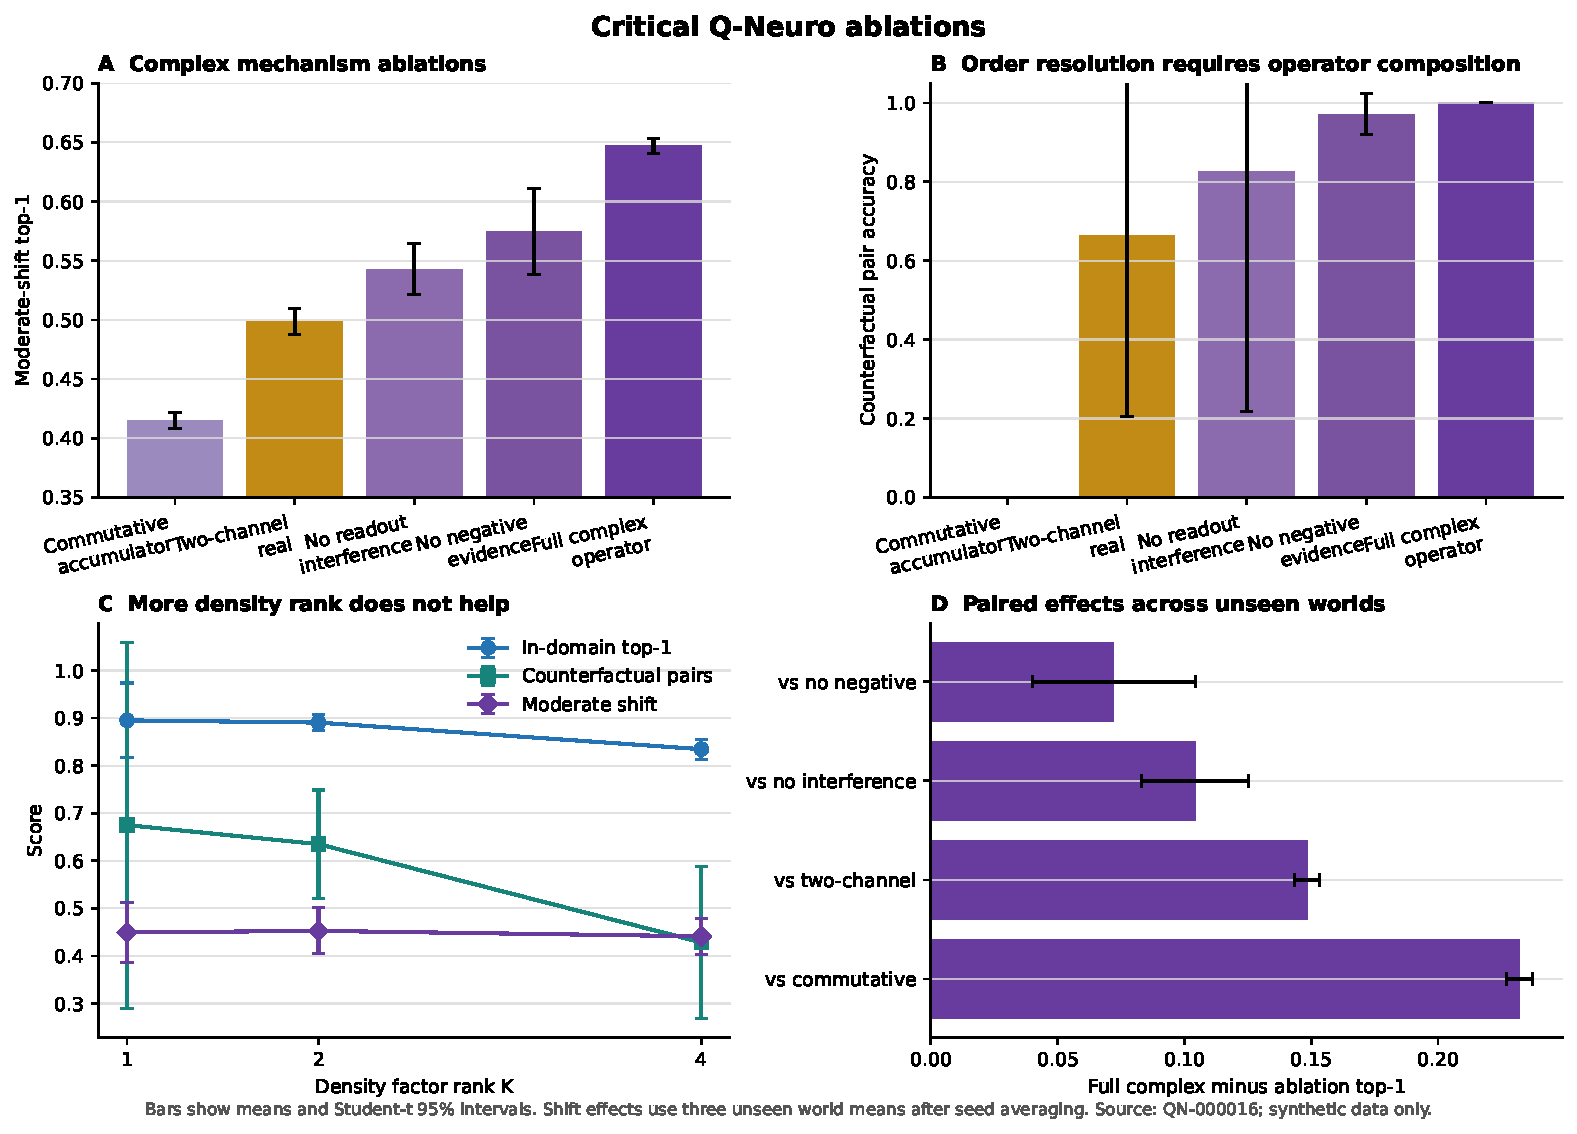
\includegraphics[width=0.98\linewidth]{figures/critical_ablation_suite.pdf}
\caption{Removing ordered composition produces the largest robustness and chronology loss. Phase-insensitive measurement and removal of observed-negative evidence also degrade the full complex model. Density rank does not improve the tested frontier.}
\label{fig:critical_ablation_suite}
\end{figure}

\input{tables/critical_ablations.tex}

\subsection{Coherence and dissipation}
The Hamiltonian-style model reaches 0.556 moderate-shift top-1 and 0.983 chronology-pair accuracy. Dissipative-only evolution reaches 0.438 and 0.008. Their hybrid reaches 0.550 and 0.923. Hybrid-minus-dissipative is +0.112 with a narrow three-world interval, while hybrid-minus-Hamiltonian is --0.006 with an interval crossing zero. Generic learned damping is not an automatic model of diagnostic elimination.

The most plausible explanation is architectural: elementwise damping plus normalization can erase path information without targeting a contradicted hypothesis. The result does not reject all dissipative or Lindblad-like laws. It rejects this generic parameterization under this objective and suggests that future dissipation must be diagnosis-conditional and compared against a matched removal operator.

\subsection{Density rank}
Density ranks one, two, and four reach 0.449, 0.453, and 0.441 moderate-shift top-1. Rank four uses more parameters but lowers source accuracy, worsens ambiguity NLL, and reduces chronology-pair accuracy. Off-diagonal capacity is therefore not automatically useful when supervision sees only the diagonal diagnosis measurement.

The invariant checks still matter: every tested density state is Hermitian, positive semidefinite, and unit trace within numerical tolerance. What fails is the predictive hypothesis. A later-resolution task or multi-observable objective could make off-diagonal structure identifiable; the present benchmark does not.

\subsection{Ambiguity differential}
The real operator’s advantage on ambiguity is not a small calibration detail. It assigns nearly four times as much mass to the valid twin set as the complex model and is much closer to the theoretical pair NLL floor. Meanwhile, the complex model leads source and shifted top-1. The result exposes a central design tension between sharp order discrimination and calibrated coexistence of unresolved hypotheses.

\begin{figure}[t]
\centering
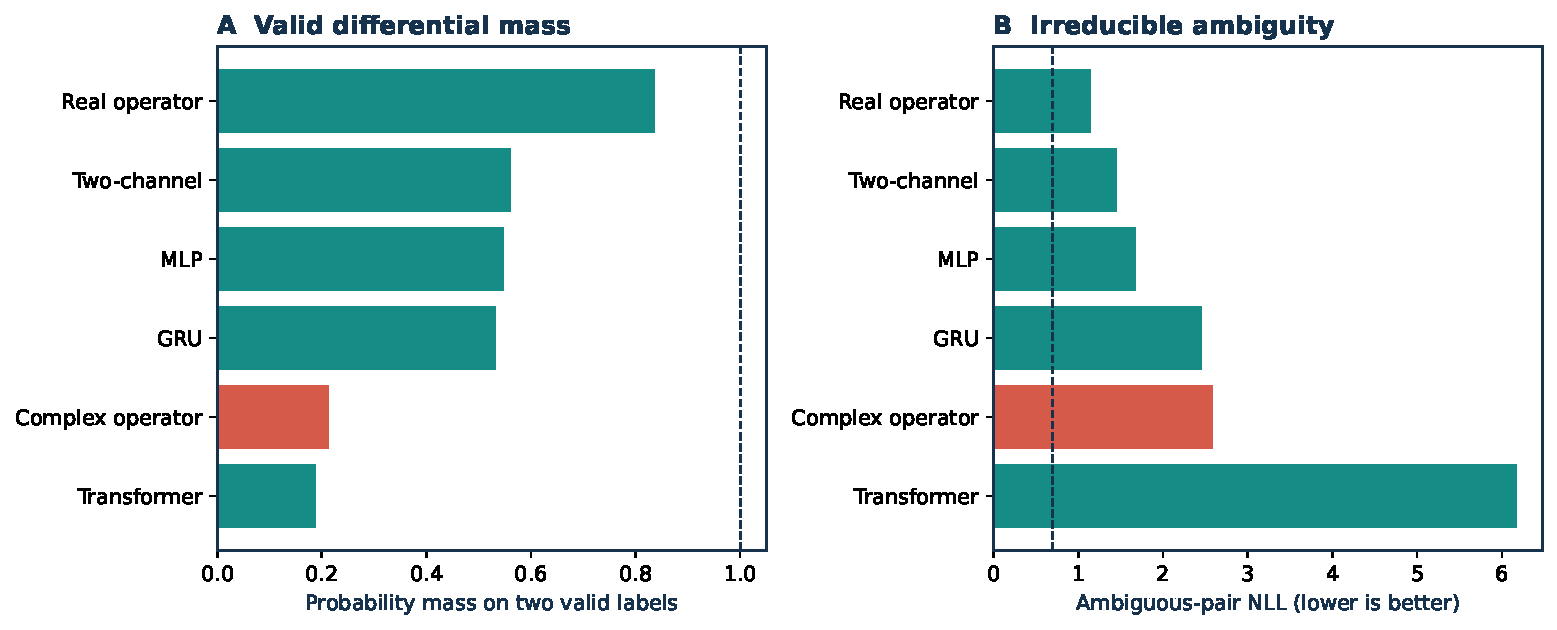
\includegraphics[width=0.98\linewidth]{figures/ambiguity_differential.pdf}
\caption{The real operator retains substantially more probability mass on the two valid ambiguity labels, while the complex operator has worse pair NLL despite stronger shifted classification accuracy.}
\label{fig:ambiguity_differential}
\end{figure}

An ambiguity-aware loss could directly supervise a valid label set or impose a distribution over equivalence classes. Such a loss would change the problem and must be evaluated for accuracy tradeoffs. The architecture alone does not guarantee metastable differentials.

\subsection{Ablation interpretation}
The ablations support a constrained mechanism chain: signed evidence enters in order; noncommuting composition preserves chronology; complex phase participates in the readout; and the resulting parameterization is robust to the declared shifts. They do not support a physical quantum interpretation, a unique representation theorem, or a claim that coherence is inherently beneficial. The density and dissipation failures are especially important because they show that adding more quantum-inspired structure can make the system worse.

% Generated from paper/source. Do not edit by hand.
\section{Interpretation of learned state}
\subsection{What exact equivalence permits us to say}
Complex coordinates can provide an economical language for rotations, relative phase, and ordered evidence updates. They may make a mechanism easier to write or constrain. In Q-Neuro, trajectories, amplitudes, entropies, state velocities, and phase-sensitive readouts are observable, and destructive interventions show dependence on several of these quantities. Exact-real equivalence means that such observables should be interpreted as coordinates of a structured dynamical system, not as evidence that the system requires intrinsically complex arithmetic.

\subsection{Probe evidence is not unique}
Earlier frozen-state probes recovered synthetic simulator factors such as mechanism, localization, temporality, and context from complex states. Conventional recurrent and state-space controls recovered the same factors as well or better. Linear decodability establishes accessibility to a probe, not causal use, disentanglement, or human interpretability. The current paper therefore treats probe results as historical mechanism observations rather than support for the primary claim.

\subsection{A more defensible explanatory object}
The strongest explanation produced by the project is the comparator transformation itself. The positive result versus the two-channel model is real within its declared benchmark. The exact block shows which part is a coordinate choice. The best-real envelope shows that the claimed advantage is not stable under control strengthening. The law failure shows that a compact post hoc pattern does not transfer. These linked artifacts explain why the scientific conclusion changed without erasing the original evidence.

\subsection{Limits of mechanistic language}
Terms such as coherence, interference, Hamiltonian, and measurement are mathematical descriptions in this repository. They do not establish a physical quantum substrate, biological plausibility, or a cognitive theory. A future mechanistic claim would require interventions that discriminate between mapped parameterizations, predeclared causal predictions, and independent replication on tasks whose generators were not designed by the project.

% Generated from paper/source. Do not edit by hand.
\section{Limitations}
\subsection{Synthetic-only evidence}
Every case in this work is generated. NeuroWorld provides exact counterfactuals and eliminates privacy risk, but it cannot reproduce the prevalence, comorbidity, documentation noise, institutional practice, measurement process, or harm asymmetry of clinical neurology. The labels are simulator archetypes rather than diseases. A model that reaches 1.000 synthetic top-1 may still be useless or dangerous on a patient. No reported number is a clinical accuracy estimate.

The generator and architecture were developed in the same project. Five unseen world seeds measure robustness to declared variations, not to an independently conceived causal process. Shared scaffolding may privilege the operator representation. The strongest result must therefore be replicated on generators built by independent teams, ideally with blinded model selection and locked analysis.

\subsection{Small replication counts}
Most studies use three training seeds because the project targets consumer hardware. World-level effects use five unseen worlds in the confirmation sweep and three worlds in several later suites. Student-t intervals summarize the observed variation but are unstable at these sample sizes. They do not quantify uncertainty over all plausible simulators, implementations, or clinical populations.

The experimental program evaluates many architectures, tasks, and metrics. Even with preregistered pairings and a claim ledger, selection pressure remains. The discovery engine is explicitly exploratory, and no proposal it emits should be treated as confirmed by the data that generated it. A future confirmatory study needs a frozen primary endpoint, independent code review, and a separately generated benchmark.

\subsection{Baseline and optimization scope}
The control set is broad for a small CPU study but not exhaustive. It does not include large pretrained clinical language models, modern long-context architectures at production scale, Bayesian neural networks, ensembles, conformal predictors, or every real-valued reparameterization of complex multiplication. Hyperparameter searches are intentionally small. The statement that the complex operator leads tested shift accuracy is not a claim that it would beat a fully tuned contemporary model.

The two-channel real operator matches width and quadratic measurement but may not match every complex inductive constraint. Complex multiplication can always be written as structured real arithmetic. The empirical question is whether the chosen parameterization helps optimization or generalization at the tested scale, not whether it computes functions inaccessible to real networks.

\subsection{Calibration and ambiguity}
The complex model is poorly calibrated in several regimes and markedly inferior to the real operator on irreducible ambiguity. Source temperature scaling worsens shifted calibration. These are not peripheral metrics: a differential system must preserve uncertainty when evidence is insufficient. Until an ambiguity-aware objective and shift-valid calibration method succeed without erasing robustness, the architecture is unsuitable for decision support even before considering data validity.

ECE itself depends on binning and can hide class-conditional errors. The repository also reports NLL, but does not yet include Brier decomposition, adaptive calibration error, conformal coverage, or decision-curve analysis. Omitted-disease AUROC is measured on one synthetic held-out class and may overstate performance when unknowns lie closer to known diagnoses.

\subsection{Compute measurement}
Training and latency are measured on one consumer MacBook CPU. Wall-clock variation, library versions, thermal conditions, and allocator caching can affect results. Peak RSS deltas are approximate. FLOPs are not analytically normalized across custom complex operations. Parameter counts are reliable; fine-grained hardware efficiency claims are not.

Hard halting shows a real reduction in executed states and latency, but all cases stop after two steps. The result is fixed truncation. The adaptive attractor never demonstrates case-dependent compute, and the sequence lengths are too short to establish long-context scaling behavior.

\subsection{Interpretability and novelty}
Factor probes show decodability, not causal use. State trajectories show computational change, not a validated medical rationale. The terms “hypothesis,” “interference,” “Hamiltonian,” and “density” are mathematical descriptions and may invite anthropomorphic or physical interpretations. The manuscript repeatedly limits those readings because attractive vocabulary can outrun evidence.

The prior-art search is extensive but non-systematic. It was performed by one investigator and one coding agent, without dual screening or a registered review protocol. Patent literature, theses, non-English work, and unpublished systems were not exhaustively searched. The paper claims a reproducible combination and evidence framework, not invention of complex networks, density states, adaptive inference, active acquisition, or local learning.

\subsection{Authorship and automation disclosure}
The project was developed by an independent researcher with assistance from an AI coding and writing agent. The agent helped implement code, run tests, structure experiments, generate figures, search prior art, and draft text. The human author remains responsible for the scientific claims, repository publication, and any future submission. Automated assistance is disclosed because provenance matters, especially in a paper about AI.

The manuscript has not undergone peer review, clinician review, independent statistical audit, or external replication. “Publication-ready” in this repository means structurally complete, reproducible, and conservatively written---not accepted, clinically validated, or award-worthy.

\input{safety}
\input{discussion}
% Generated from paper/source. Do not edit by hand.
\section{Conclusion}
Q-Neuro tests whether an ordered complex hypothesis state is a useful computational bias for sequential synthetic diagnosis. Across a registered program of corrected baselines, unseen worlds, orthogonal tasks, eighteen dynamical laws, ablations, probes, training laws, hard execution, and trajectories, one result persists: the complex operator is more robust than the tested real and conventional controls under the declared NeuroWorld shifts, and order, phase-sensitive measurement, and negative evidence each contribute.

The same evidence rejects a general superiority claim. GRU is more source-data-efficient, real operators are much better on irreducible ambiguity, source calibration does not transport, OOD separation is not unique, adaptive depth degenerates, and unconventional learning laws do not improve the frontier. Complex dynamics are a conditional tradeoff, not a universal replacement for neural networks.

The scientific contribution is a reproducible way to ask the question without hiding the answer’s boundaries. Every table and figure is generated from registered artifacts; failed ideas and superseded runs remain visible; the paper, Word document, PDF, dashboard, and repository are synchronized. The next claim must come from independent causal replication, not stronger language applied to the same simulator.

\input{appendices}
\clearpage
\bibliographystyle{unsrtnat}
\bibliography{references}
\end{document}
